% figures/CRI-manuscript_figure_1.tex
\documentclass[tikz,border=2pt]{standalone}

\usepackage{amsmath}
\usepackage{tikz}
\usetikzlibrary{arrows.meta,positioning,calc,fit,shadows.blur,backgrounds,decorations.pathmorphing}
\usepackage{pgfplots}
\pgfplotsset{compat=1.17}

\newcommand{\T}{T}

\tikzset{
  kern/.style={rectangle, rounded corners=2mm, minimum width=28mm, minimum height=13mm,
               draw=black, line width=0.5pt, align=center, font=\small,
               top color=white, bottom color=gray!5, blur shadow},
  chan/.style={rectangle, rounded corners=2mm, minimum width=38mm, minimum height=15mm,
               draw=black, line width=0.5pt, align=center, font=\small,
               top color=white, bottom color=gray!5, blur shadow},
  gatebox/.style={rectangle, rounded corners=2mm, minimum width=40mm, minimum height=15mm,
                  draw=black, line width=0.6pt, top color=yellow!15, bottom color=yellow!5,
                  align=center, font=\small\bfseries, blur shadow},
  futcircle/.style={circle, minimum size=28mm, inner sep=0pt, fill=white,
                    preaction={draw=green!70!black, line width=6pt},
                    draw=red!75!black, line width=0.9pt},
  arr/.style={-Latex, line width=0.9pt},
  darr/.style={-Latex, line width=0.9pt, dashed, color=purple!70!black},
  title/.style={font=\bfseries},
  tinycap/.style={font=\scriptsize, inner sep=1pt, text opacity=0.9},
  badge/.style={rectangle, rounded corners=1.5pt, inner sep=2pt, font=\scriptsize\bfseries,
                draw=black, fill=black!5}
}

\begin{document}

\begin{tikzpicture}[node distance=20mm, xshift=-25mm]

% Top row
\node[kern, fill=teal!8, draw=teal!60!black] (mem)
  {$\mathbf{D_{\mathrm{mem}}[\rho(t)]}$\\[-1mm]\scriptsize $\displaystyle \int_{0}^{\infty}K(s)\,\rho(t-s)\,ds$};
\node[kern, fill=blue!8, draw=blue!60!black, right=of mem, xshift=10mm] (sens)
  {$\mathbf{D_{\mathrm{sens}}[\rho(t)]}$\\[-1mm]\scriptsize Markovian};

% Future as circle with thick outer green ring
\node[futcircle, right=of sens, xshift=10mm] (fut)
  {$\mathbf{D_{\mathrm{future}}[\rho(t)]}$};
\node[tinycap, below=1.5mm of fut]
  {$\displaystyle \int_{0}^{T_0} w(\tau_f,t)\,\mathcal{D}\!\big[L_{b,f}(\tau_f)\big]\,\rho(t)\,d\tau_f$};

% Gate
\node[gatebox, above=of sens, yshift=12mm] (gate)
  {Goldilocks Gate\\[-0.5mm]\(\displaystyle G\!\big(P(\tau_f)-p_0(a(t))\big)\)};

\draw[arr] (mem) -- node[midway,above,sloped,tinycap]{\(\textstyle K(s)\)} (sens);
\draw[arr] (sens) -- (fut);

\draw[darr] (gate.east) .. controls +(1.3,0.0) and +(-0.6,1.2) .. (fut.north)
  node[pos=0.45, below=7pt, xshift=8pt, text=purple!70!black, font=\scriptsize]
  {$\displaystyle w(\tau_f,t)=\kappa_w(t)\,G\!\big(P(\tau_f)-p_0(a(t))\big)\,e^{-\tau_f/\tau_{\mathrm{fut}}}$};

\node[title, above=9mm of gate] {Kernel interactions};

% Right insets
\node[draw=black, line width=0.4pt, rounded corners=1mm, fill=yellow!5, inner sep=2pt, right=6mm of fut] (inset1) {
\begin{tikzpicture}
  \begin{axis}[width=3.6cm, height=2.4cm, xmin=0, xmax=1, ymin=0, ymax=1,
    xtick={0,0.5,1}, ytick={0,0.5,1},
    ticklabel style={font=\tiny}, label style={font=\tiny},
    every axis plot/.append style={line width=0.9pt},
    axis lines=left, title style={font=\scriptsize}, title={\scriptsize Gate \(G(x)\)}]
    \addplot [domain=0:1, samples=200] {1/(1+exp(-(x-0.5)/0.08))};
    \node[font=\tiny] at (axis cs:0.5,0.12) {$p_0(a)$};
    \draw[dashed] (axis cs:0.5,0) -- (axis cs:0.5,1);
  \end{axis}
\end{tikzpicture}
};
\node[draw=black, line width=0.4pt, rounded corners=1mm, fill=blue!5, inner sep=2pt, below=3mm of inset1] (inset2) {
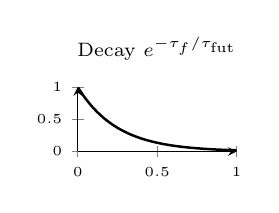
\begin{tikzpicture}
  \begin{axis}[width=3.6cm, height=2.4cm, xmin=0, xmax=1, ymin=0, ymax=1,
    xtick={0,0.5,1}, ytick={0,0.5,1},
    ticklabel style={font=\tiny}, every axis plot/.append style={line width=0.9pt},
    axis lines=left, title style={font=\scriptsize},
    title={\scriptsize Decay \(e^{-\tau_f/\tau_{\mathrm{fut}}}\)}]
    \addplot [domain=0:1, samples=200] {exp(-x/0.25)};
  \end{axis}
\end{tikzpicture}
};
\node[tinycap, right=1mm of inset1] {gate on partial cumulative \(P(\tau_f)\)};
\node[tinycap, right=1mm of inset2] {future decay with time constant \(\tau_{\mathrm{fut}}\)};

% Badges
\coordinate (badgeY)  at ($(fut.north east)+(0,12mm)$);
\coordinate (badgeY2) at ($(badgeY)+(0,-6mm)$);

\node[badge, anchor=south] (badge1) at ($(inset1.center |- badgeY)$)
  {$p(\tau_f)$: density [s$^{-1}$] \ \ $P(\tau_f)=\int_0^{\tau_f}\!p(u_f)\,du_f\in[0,1]$};

\node[badge, anchor=south, yshift=-3mm] (badge2) at ($(inset2.center |- badgeY2)$)
  {$\kappa_w(t)$: [s$^{-1}$] \ \ $\displaystyle \gamma_b(t)=\int_0^{\T_0}\!w(\tau_f,t)\,d\tau_f$};

% Bottom row (reduced surrogate)
\node[title, below=16mm of sens] (title2) {Reduced surrogate (single effective retro-rate)};
\node[chan, fill=gray!7, draw=black!70, below=6mm of title2] (collapse)
  {$\displaystyle \gamma_b(t)=\int_0^{\T_0}\! w(\tau_f,t)\,d\tau_f$};
\node[kern, fill=magenta!10, draw=magenta!60!black, right=of collapse, xshift=6mm] (Lb)
  {$\mathbf{D_{b}[\rho(t)]}$\\[-0.5mm]\scriptsize single jump w/ rate $\gamma_b(t)$};
\node[kern, fill=blue!10, draw=blue!60!black, right=of Lb, xshift=6mm] (fwd)
  {$\mathbf{D_{\mathrm{fwd}}[\rho(t)]}$\\[-0.5mm]\scriptsize control (time-local)};

\begin{scope}[on background layer]
  \draw[arr, preaction={draw=white, line width=3pt}]
    (fut.south) to[out=270, in=0] (collapse.east);
  \draw[arr, preaction={draw=white, line width=3pt}] (collapse) -- (Lb);
  \draw[arr, preaction={draw=white, line width=3pt}] (Lb) -- (fwd);
\end{scope}

\node[tinycap, below=4mm of Lb]
  {collapse of continuum \(\{L_{b_f}(\tau_f)\}\) to \(L_b\) with rate \(\gamma_b(t)\) (see SI)};

\end{tikzpicture}

\end{document}
